\chapter{Une piste de solution : l'augmentation de la natalité}
\paragraph{}Dans le premier chapitre nous avons vu que le taux de natalité oscille entre 1,5 et 1,7 en moyenne dans l’Europe des 28 aux cours des quinze dernière année, alors que le seuil de renouvellement se situe autour de 2,1~\citep{eur-lex}. Si la population européenne continue de croître, c’est donc uniquement dû à l’immigration.  La première question que nous posons cherche à savoir si l’augmentation du taux de natalité pourrait être une solution contre le vieillissement de la population. Ensuite, si oui, dans quelle mesure ce taux de natalité devrait-il augmenter? Enfin, quelle mesure pourrait-on adopter pour que le taux de natalité augmente, étant évident qu'on ne peut simplement l'imposer?
\section{L'augmentation de la natalité : une vraie solution ?}
\paragraph{}L’article de Héran~\citep[pp.1]{heran} répond à la première partie de la question lorsqu’il parle d’une part évitable et d’une part inévitable du vieillissement de la population. La part inévitable est due au baby boom et à l’accroissement de la durée de vie. La part évitable est le vieillissement par le bas qui peut être ralenti. L’article de Héran~\citep[pp.5-6]{heran} détaille pour chaque pays d’Europe l’évolution des jeunes (0-14 ans), de la population active (15-64 ans), et des personnes agées (+65 ans). Nous n’avons repris dans le graphe \ref{vieillissement} que la France et l’Allemagne car ces deux pays représentent respectivement un taux de natalité très élevé (2,01) et très faible (1,42) par rapport à la moyenne européenne. Pourtant, les deux pays voient leur population de personnes âgées augmenter de 80\% de 2000 à 2015. Cela représente la part inévitable du vieillissement comme nous l'avons vu au chapitre 1. Part contre on peut observer une diminution de 20\% du reste de la population sur le même laps de temps en Allemagne alors que celle-ci reste stable en France. 

\begin{figure}[h!]
    \begin{center}
        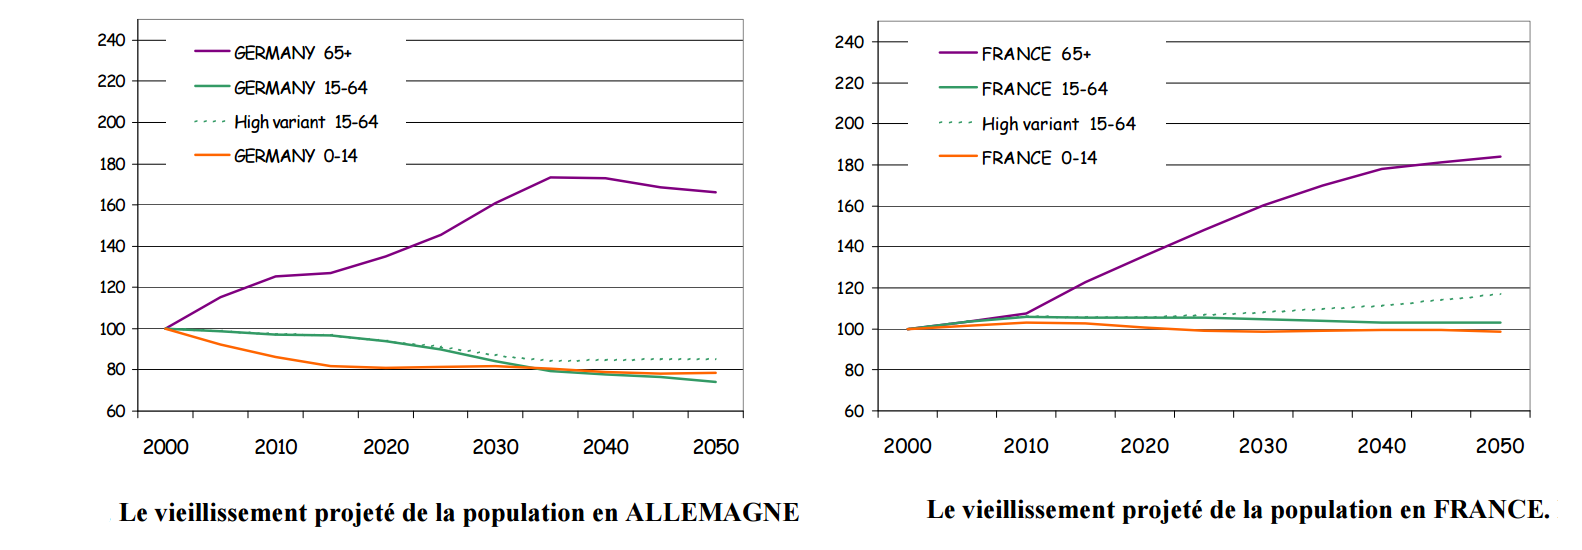
\includegraphics[scale=0.4]{document/vieillissement.png}
        \caption{Source: Héran~\citep[pp.5-6]{heran}}
        \label{vieillissement}
    \end{center}
\end{figure}

La Figure~\ref{FR-DE_natalite.png} montre les projections d’Eurostat~\citep{eurostat_europop13} pour les deux pays de 2015 à 2080. Le graphe de gauche représente le scénario sans immigration. Dans ce scénario, on peut observer que malgré une augmentation du taux de natalité à 1,7, l’Allemgane perd 30 millions d’habitants alors que la France croît d’abord légèrement pour se stabiliser vers 70 millions. Dans scénario principale d'Eurostat~\citep{eurostat_europop13}, l'immigration ne fait qu’atténuer la perte d’habitants pour l’Allemagne alors que la France gagne presque 15 millions d’habitants. L’augmentation de la natalité est-elle une solution au vieillissement de la population ? Non, elle ne pourra pas contrecarrer les effets du Baby Boom et de l’augmentation de l’espérance de vie. Mais elle reste indispensable sur le long terme pour le maintient de la population à son niveau actuel, car l’immigration à elle seule ne permettra pas non plus le maintien de la population. Si le taux de natalité se situe proche du seuil de renouvellement, la pyramide des âges finira pas s'équilibrer et à ressembler à un cylindre, une fois l’effet du Baby Boom passé après 2050. L’augmentation du taux de natalité doit se maintenir dans le temps et ne plus redescendre, sinon nous pourrions nous retrouver en face d’un nouvel effet Baby Boom. 
\newpage
\begin{figure}[h!]
    \begin{center}
        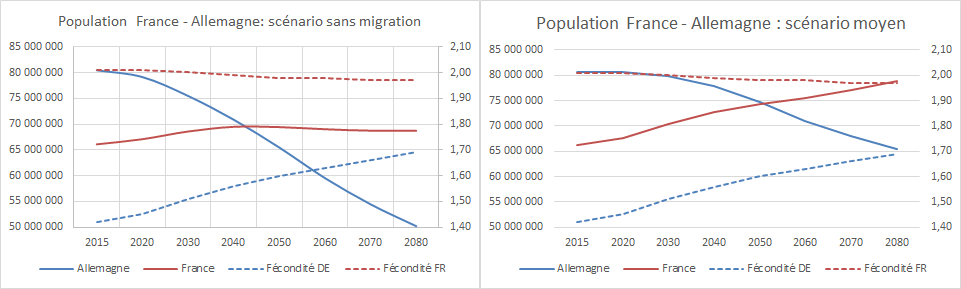
\includegraphics[scale=0.70]{document/FR-DE_natalite.png}
        \caption{Source: Eurostat~\citep{eurostat_europop13}}
        \label{FR-DE_natalite.png}
    \end{center}
\end{figure}

\section{Les causes d'un faible taux de natalité}
\paragraph{}Il faut ensuite se demander pourquoi le taux de natalité est faible dans des pays comme l’Allemagne ou les pays du sud (Espagne, Italie, Portugal)~\citep{4model}, et quelle politique pourrait favoriser une augmentation de ce taux. 

\paragraph{}Pour Le Bras, la raison économique est sans doute la plus simple : la difficulté à accéder à un emploi à pour effet de diminuer la fécondité~\citep[pp.25]{heran}, les femmes repartissant leurs efforts entre emploi et famille. Si trouver et maintenir un emploi nécessite beaucoup d’efforts, il ne reste plus d’énergie à consacrer à la famille. De plus, étonnamment, on remarque dans les pays plus traditionnels comme l’Espagne, le Portugal ou l’Italie, que le fait d’avoir une proportion importante de femmes au foyer diminue le taux de fécondité. Il a pu établir une corrélation entre le taux de fécondité et le taux d'activité des femmes. 

\paragraph{}L’Allemagne est une exception par rapport aux autres pays du nord qui possède un meilleur taux de fécondité. Une mentalité très rigide en matière de famille, où la mère doit prendre en charge les enfants, fait qu'elle culpabilise si elle doit continuer à travailler. Il y a d’ailleurs un terme pour ces femmes en Allemagne : RabenMutter~\citep{mutter}. 

\paragraph{}Le rapport Roy~\citep{quebec} décrit les trois conditions nécessaires à la venue d’un enfant au sein d’un couple : la sécurité financière, une relation stable et sûre, et un conjoint qui partage les tâches ménagères~\citep[pp.19]{quebec}. Il expose aussi plusieurs théories afin d'expliquer un faible taux de fécondité. La première, la théorie du choix rationnel, considère la mise en balance des coûts directs et indirects\footnote{Parmis les coût indirects, on peut citer le fait de devoir quitter son travail ou de travailler à mi-temps, ou encore une pause carrière alors que les coût directe représente les sommes d'argent dépenser pour l'enfant, sa nourriture, sa garde et les soins à lui prodiguer.} de l’enfant d’un coté, et l’avantage psychologique de l’autre. S'il est certes possible de faire peser plus l’avantage psychologique en influençant les mentalités, il est plus facile de diminuer le poids des coûts directs et indirects lié aux enfants~\citep[pp.23]{quebec}. La seconde théorie du rapport Roy est celle de l’évitement du risque, selon laquelle les coûts associés au fait d’avoir des enfants sont certains, alors que les bénéfices qu’on va en tirer ne sont qu'hypothétiques. Lorsque l'avenir personnel est incertain, les gens vont se tourner vers le choix le moins risqué : l’absence d’enfant~\citep[pp.24]{quebec}. La troisième théorie est celle de l'inadéquation de l’équité des sexes au travail et à la maison~\citep[pp.25]{quebec}. Selon cette théorie, si il y a inadéquation entre l'égalité au travail et à la maison. C'est-à-dire que la femme travail aussi mais malgré tout elle reste la seule à s'occuper des tâches ménagères. Cela représenterait un poids trop lourd pour envisager la maternité.

\section{Les politiques possibles pour encourager la natalité}
\paragraph{}Au vu de ces théories, il apparaît plus clairement quelles politiques pourraient favoriser une augmentation de la natalité. L’objectif de ces politiques seraient de lever les obstacles à la décision d’avoir un enfant. Elle devrait selon Roy~\citep[pp.43-46]{quebec}:

\begin{itemize}
  \item favoriser l’emploi car, comme nous l’avons vu, la facilité d’accès à l'emploi pour les femmes favorise la fécondité, et l’emploi reste le meilleur facteur de stabilité financière.
  \item favoriser la conciliation du travail et de la famille, qui pourrait se concrétiser par les mesures suivantes : congés parentaux, accueil des enfants dès la fin des congés parentaux, horaires de travail plus souples, égalité des sexes au travail.
  \item compenser les coûts générés par un enfant, car ils représentent le meilleur investissement pour une société. Or la famille permet la naissance de cette investissement, un service qui devrait être rémunéré. Parmi ces mesures, on peut citer des allocations familiales, les allocations pour la scolarité, des avantages fiscaux pour les parents et des services gratuits pour les familles.
  \item favoriser un changement de mentalité, absolument nécessaire en Allemagne, favoriser les attitudes positives envers les enfants et les parents, promouvoir une égalité des sexes aux travail mais aussi à la maison. 
\end{itemize}

\paragraph{}Pour finir, selon Héran, il est important que les mesures prises en faveur de la famille soient inscrites dans la durée et subsistent aux alternances politiques car les futurs parents doivent pouvoir bénéficier d’une politique stable tout au long de l'éducation de leurs enfants~\citep[pp.14]{heran}. 

\paragraph{}Malgré cela, la conclusion de Le Bras n’est pas très optimiste : “il faut renoncer à l’idée d’assister rapidement à une reprise de la fécondité en Europe”~\citep[pp.27]{heran}. Pour lui, deux modèles de fécondité se partagent l’Europe : un modèle basé sur l’intervention de l’état dans les pays du nord et en France, et un modèle centré sur le rôle de la famille. Les mesures qui favorisent la fécondité ne seraient pas l'origine de ces deux modèles, mais leurs conséquences. S’il est relativement facile de changer les politiques familiales, il l’est beaucoup plus de changer les mentalités ancrées dans une société. Il faut du temps et les effets ne se feront resentir qu'à long terme : “La France a mis cent ans à tirer le bénéfice de sa législation nataliste.”\citep[pp.28]{heran}

\paragraph{}Nous avons vu que l’augmentation de la natalité permettrait un maintien de la population en Europe à long terme et, allié à une immigration constante, conduirait à un accroissement de la population et à une stabilisation de l'âge moyen de la population. Mais il faut se rendre à l’évidence, cette approche n'apportera aucune solution à court terme ; elle doit donc être combinée à d’autre solutions.  
